\documentclass[12pt]{article}

\title{Constraining the Supersonic Relative Velocity Effect on the Baryon Acoustic Oscillation Peak}
\author{Jenna Freudenburg \\
                Adviser: Nikhil Padmanabhan\\
                Yale University
}
\date{\today}

\usepackage{graphicx}
\usepackage{float}

\begin{document}
\maketitle

\begin{abstract} 
As a participant in Independent Projects in Physics, I have spent this semester working with Prof. Nikhil Padmanabhan. The goal of this project is to refine existing models for calculating the peak in the galaxy correlation function caused by baryon acoustic oscillations.
\end{abstract}
\tableofcontents

\section{Background}
\subsection{The primordial universe and the baryon acoustic oscillations}

The early universe consisted of primordial plasma, first composed of quarks and gluons and later of free baryonic particles that interacted with photons via Thompson scattering. At approximately $3\times10^{5}$ years after the Big Bang, the universe had cooled to ~3000 K. This point marks the era of recombination, at which time the baryons formed neutral hydrogen and Thompson scattering was suppressed. Up until this point, anisotropies in the cosmic fluid resulted in gravitational forces variations that competed with pressure from the photon-baryon interactions to create acoustic oscillations \cite{Eisenstein}. At recombination, the matter and photons ceased to interact, and the photons free-streamed throughout the universe, which we see today as the cosmic microwave background. This left propagating overdensities of baryons essentially fixed at the sound horizon. Over time, these overdensities accreted gravitationally to form galaxies, and thus by measuring galactic positions today, we can detect this horizon and use it as a characteristic cosmic length scale. This provides a standard ruler that can be use to measure cosmic acceleration independent of supernovae standard candles (which have been used in the past for cosmic measurement), and as such the BAO provides an important tool for the study of dark energy. Studies have calculated the correlation function over large galaxy samples from the Sloan Digital Sky Survey (SDSS) and found a peak attributable to the BAO at about 150 Mpc separation \cite{Eisensteinetal}.

\subsection{The supersonic relative velocity effect}

In a recent study \cite{Yooetal}, Yoo et al. investigate the implications of nonlinear contributions to the BAO feature. Specifically, they analyze the proposition that the supersonic velocity of the dark matter fluid relative to the baryonic fluid after recombination impacts the evolution of the BAO feature. In theory, this relative velocity should raise the effective Jeans mass (the critical mass at which a cloud of matter collapses under gravity) and thus delay the formation of baryonic structure. Such a delay in structure formation would alter the power spectrum measured over galaxies that exhibit the effect, and thus shift the BAO peak.

\section{Calculations}
\subsection{Summary of progress **}

This semester, I have continued to confirm the model presented in Yoo et al. Specifically, the higher-order terms that appear in the power spectrum as a result of including the supersonic relative velocity effect have been confirmed. Following Yoo et al., we assume a second-order term in the galaxy density fluctuation as follows:

$$\delta_{g}=b_{1}\delta_{m}({\bf x})+b_{r}[u_{r}^{2}({\bf x})-\sigma_{ru}^{2}]$$

where $u_{r} ={\bf v}_{r}/\sigma_{rv}$ and $\sigma_{rv}$ is the one-dimensional rms relative velocity fluctuation. Using perturbation theory, the equation for the full power spectrum is calculated to be 

$$P_{g}(k) = b_{1}^{2}P_{nl}({\bf k}) + \int\frac{d^{3}\bf q}{(2\pi)^{3}}P_{m}(q)P_{m}(|{\bf k - q}|)[\frac{1}{2}b_{2}^{2}+2b_{1}b_{2}F_{2}({\bf q, k- q})$$
$$+4b_{1}b_{r}F_{2}({\bf q, k- q})G_{u}({\bf q, k- q})+2b_{2}b_{r}G_{u}({\bf q, k- q})+2b_{r}^{2}G_{u}({\bf q, k- q})^{2}]$$

where $F_{2}$ and $G_{u}$ are the density field and velocity divergence field kernels, respectively \cite{Yooetal} \cite{Bernardeau}.

\subsection{Power spectrum}
\begin{figure}[H]
	\centering
	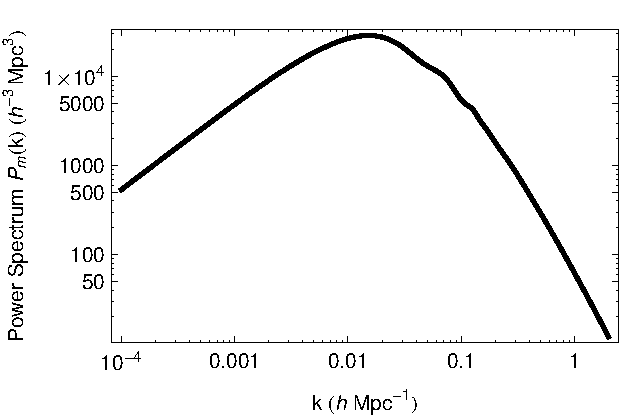
\includegraphics[width=12cm]{Pm}
	\caption{The linear matter power spectrum.}
	\label{Pm}
\end{figure}

\subsection{Bispectrum}
\begin{figure}[H]
	\centering
	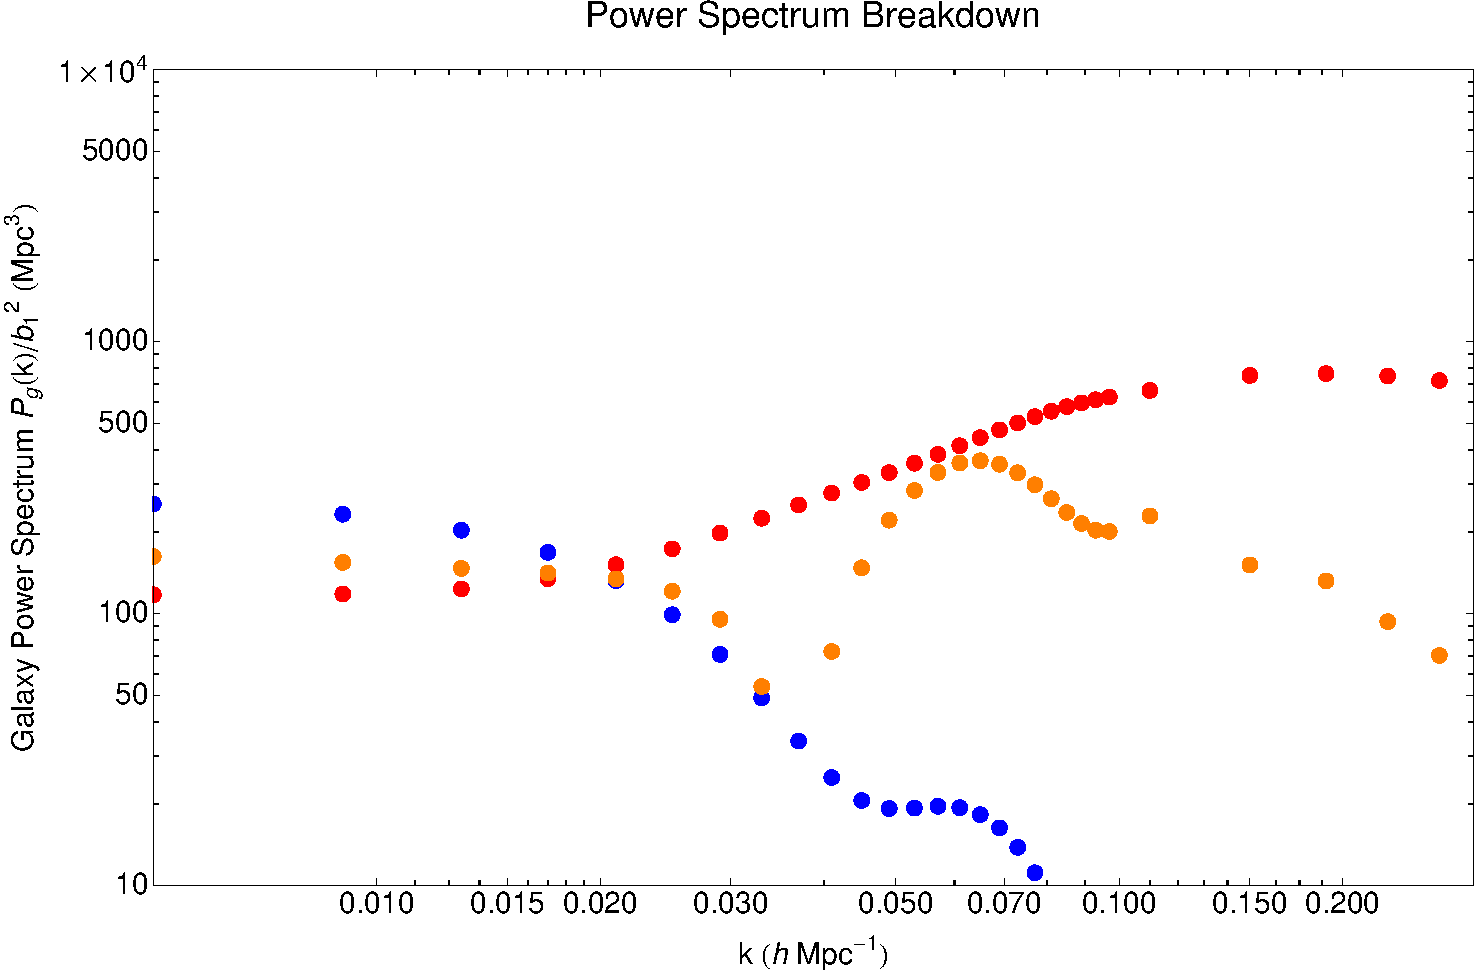
\includegraphics[width=13cm]{PSbd}
	\caption{The full galaxy power spectrum (blue = auto-relative velocity term, orange = cross power terms, red = matter terms).}
	\label{PSbd}
\end{figure}

We compare this linear power spectrum to the full power spectrum, given above, which includes second order terms from both the matter density and the relative velocity fluctuations. Figure \ref{PSbd} breaks down the full power spectrum term by term, and shows the clear deviation that these higher-order terms cause in the galaxy power spectrum. 

\section{Discussion and conclusions}

From merely confirming the results of Yoo et al., I have now begun to analyze their results independently. A linear matter power spectrum, represented above as $P_{m}$, was obtained from data generated from a fiducial cosmology using CAMB (Code for Anisotropies in the Microwave Background). This result is shown in Figure \ref{Pm}.

\subsection{Future work**}

I have now begun to apply these results to data from large-scale cosmology simulations. I plan to first run the full power spectrum that I have constructed through a set of 600 "mock" galaxy catalogs, which will allow me to gather a critical level of statistics. The results of this simulation will allow me to calculate the offset in the BAO feature caused by the supersonic relative velocity effect for various values of $b_{2}$, and $b_{r}$ (which are unknown parameters corresponding to the second-order density fluctuations). Ultimately, I plan to run the simulation using real data from the Sloan Digital Sky Survey, and to compare the results to the predictions of Yoo et al.

\begin{thebibliography}{1}

\bibitem{TsHirata}
D. Tseliakhovich and C. Hirata, \emph{Relative velocity of dark matter and baryonic fluids and the formation of the first structures}, Phys. Rev. D \textbf{82}, 083520 (2010).

\bibitem{Eisensteinetal} 
D. Eisenstein et al., \emph{Detection of the baryon acoustic peak in the large-scale correlation function of SDSS luminous red galaxies}, Astrophys. J. \textbf{633}, 2 (2005).

\bibitem{Yooetal} 
J. Yoo, N. Dalal, and U. Seljak, \emph{Supersonic relative velocity effect on the baryonic acoustic oscillation measurements}, J. Cosmol. Astropart. Phys. \textbf{7}, 018 (2011). 

\bibitem{Szapudi}
I. Szapudi, \emph{Three-point statistics from a new perspective}, Astrophys. J. \textbf{605}, 2 (2004).

\bibitem{Eisenstein}
D. Eisenstein, "Proceedings of 'Probing the Dark Universe with Subaru and Gemini'". November 6-9, 2005 AGENDA Waikoloa, Hawaii. http://www.noao.edu/meetings/subaru, p.9.1

\bibitem{Bernardeau}
F. Bernardeau et al., \emph{Large-Scale Structure of the Universe and Cosmological Perturbation Theory}, arXiv:astro-ph/0112551v1 (2001).

\end{thebibliography}

\appendix
\section{Simulation details}


\end{document}